\documentclass[12pt]{article}
\usepackage[babel=true]{csquotes}
\usepackage{cite}
\usepackage{epigraph}
\usepackage[toc]{glossaries}
\usepackage{tikz}
\usepackage{listings}

\lstset{language=Python}

\usetikzlibrary{calc,trees,positioning,arrows,fit,shapes,calc}

\graphicspath{{../img/}}

\newacronym{rug}{RUG}{Railster Universal Gateway}
\newacronym{ui}{UI}{User Interface}
\newacronym{op}{O.P.}{Output Provider}
\newacronym{afa}{AFA}{Alternate Finite Automaton}
\newacronym{fsm}{FSM}{Finite State Machine}
\newacronym{dfa}{DFA}{Deterministic Finite Automaton}
\newacronym{nfa}{NFA}{Non-Deterministic Finite Automaton}
\newacronym{io}{I/O}{Inputs/Outputs}
\newacronym{dtmc}{DTMC}{Discrete-Time Markov chain}
\newacronym{mdp}{MDP}{Markov decision processe}
\newacronym{pa}{PA}{Probabilistic Automata}
\newacronym{ctmc}{CTMC}{continuous-time Markov Chain}
\newacronym{pta}{PTA}{Probabilistic Timed Automata}
\newglossaryentry{railsteros}
{ name=RailsterOS,
  description={A set of sub-program running on the \gls{rug} defining the behavior of it}
}
\newglossaryentry{daemons}
{ name=daemons,
  description={Sub-programs running inside \gls{railsteros} adding functionalities to it}
}
\makeglossaries

\begin{document}

\title{Practical case of Black-box driven verification}
\author{Thomas Van Gysegem}
\date\today
\maketitle

\section*{abstract}

This paper will describe a practical case of software testing and explain all the choices that where made during the implementation process. It will also try to provide some generic way of doing the same for a different use case given a similar running environment and constraints.

\clearpage
\pagebreak
\hspace{0pt}
\vfill
\epigraph{Program testing can be a very effective way to show the presence of bugs, but it is hopelessly inadequate for showing their absence}{Edsger W. Dijkstra , The Humble Programmer (1972)}
\vfill
\hspace{0pt}
\pagebreak

\clearpage

\tableofcontents

\clearpage

\section{Introduction}

There are a lot of available softwares nowadays but have you ever wondered where they all come from ? All of them comes from some developpement process. Those processes can last for days, months or even years before producing the expected software and during this process, some errors can be made that makes the software faulty or broken. That's why, all along this process, we need to make sure that everything is working just fine. To do that, we introduce a step in the developpement process called "testing". Without it, no complicated software will be able to do its task without problems. Of course, this testing step can be done differently depending on the overall developpement process but nevertheless, every software need to goes through that step.\\

Not so surprisingly, this paper is all about this particular testing step. The goal of it will be to provide a way of automating this step. As we will explain later on, providing this automatic process is of major interest in term of time gained in the developpement process and fiability for the final software. Of course, detecting all problems during tests is a really complex tasks and the process developped here will only help to reduce the risk of shipping faulty softwares and to make sure that previously encountered/corrected problems are not re-introduce between different versions of it.\\

To guide us during this work, we will focus on a concrete case study that was encountered at the Railnova company in Brussels. Of course, as the goal of this work is to stay generic, we will go from the concrete example's solution to more generic solutions that can easilly be extended for any other software.\\

Despite the fact that this paper will try yo stay generic, we will not talk about hardware testing even if we can see that as a particular case of testing in a developpement process. Despite the fact that strong timing constraint doesn't allows us to performs this hardware analysis, we think that focussing on software developpement will help the reader to get a better understanding of the principles used and developped ideas.\\

I tried to divided this work in many big parts that introduces themself one after the other. As this topic and all the techniques involved are closely related, there will often be references to area not already covered during the sequential reading of this paper.\\

The first part of this work will describe the existing techniques in software testing and discuss of what are some of the motivations of this work to introduce \gls{fsm} and how they work. Following this, we will discuss about the work that was done, why it is an important improvement and what are the decisions that lead us to this particular implementation. Then, we will explain how we designed the testing process and finally, we will describe how our particular case was handled by explaining how we integrated every inputs and outputs of our software into our testing process. We'll also give a more summarized/generic way of doing the same work for any kind of inputs and outputs.


%------------------------------------------------------------------------%
%                                                                        %
%                                                                        %
% PRELIMINARIES                                                          %
%                                                                        %
%                                                                        %
%------------------------------------------------------------------------%

\clearpage
\part{Preliminaries}

To begin with, we will present the very basics of software testing, what are the common practices and how we uses them nowadays. This will allows us to introduce the technical terms used all along this paper. Following this technical introduction, we will present the studied case that was the starting point of this work at the Railnova company to introduce \gls{fsm}. Finaly, we will describe what is a \gls{fsm} exactly and some of its variations.

\clearpage
\section{Software development and software testing}

Software development is a complex area and a lot of differents processes exists but at the very last, they all have some key principles in common. One of them being the testing part. For this work to be fully understood, we need to introduce a bit of software development and then, explain which are the different techniques used in software testing. This will provide us the required technical vocabulary to describe our own testing process.

Software development can be defined in a lot of differents ways, every one of them being more or less equivalent but in this work, we will focus on the basis and simply say that software development is some kind of plan to produce a given software. This plan can be more or less complex and must involves at some point, some testing steps.\\

Software are usually ordered by a client that can be ourself, some company or any set of users~\cite{SoftwareDevelopment:2016}. Clients have needs and our task as software developer will be to fullfill them by producing a software. The client's will first be translated into requirements specifications that, to put it simply, are formal description of them. We usually create those requirements specifications during meeting with client, this requires a lot of talk to be sure that the idea we get from them is what they want.\\

Then the software can be built. Of course, if we got the wrong requirements specifications, our software will not be what the client asked and therefore, they will want us to start again from scratch. Lets assume that those requirements are good, then, once the software is built, we want to test it to ensure that it works and that it meets the given requirements. Once those test are succesfully passed, we can ship the software to our client.\\

This whole process, starting from the client order to the shipping of the produced software is what we call the software development process. Of course, there is not one only way of doing it even for the most simple process like this one their can be divergence of workflow from one team to another. Lets introduce some of them~\cite{IIS2:IIS202348}.

\subsection{Waterfall}

The waterfall model is probably the most basic development process still used today, it is often attributed to Winston Walker Royce in a paper from 1970~\cite{BARYWBoehm:1987}. The whole process is sequential or plan driven. The whole process is divided in big part and each of them is done only one time and one after the other. The original model was designed as follows:\\

\begin{itemize}

\item System and software requirements: captured in a product requirements document
\item Analysis: resulting in models, schema, and business rules
\item Design: resulting in the software architecture
\item Coding: the development, proving, and integration of software
\item Testing: the systematic discovery and debugging of defects
\item Operations: the installation, migration, support, and maintenance of complete systems

\end{itemize}

Of course, this process is very risky and organizations tends to avoid it when possible. Between the first and the last step of it, there can be a lot of weeks, months or years ! During this time, the project needs can evolve and then, the delivered product will only match outdated requierements. Which, of course, is not a good thing for the client.\\

If some problems occurs during the writting of the product requierements, lets say that the client forgot to talk about a key feature. Then, again, the product we will deliver will miss that feature. Producing the wrong product is really a big problem of this methodology.\\

Despites those well known problems, there is still a lot of qualities to this process. As the first steps are strongly related to documentation of the product, if a team member leaves during the process, we have less risk of loosing knowledge of what has been done or what is left to do. New team members will simply need to read the requierements, the produced models and the software architecture.\\

This process is also one of the most easiest to understand, every step of the project is well documented and one can easily jump in any project using this methodology and be ready to participate in a realy small amount of time.\\

\begin{figure}
    \centering
    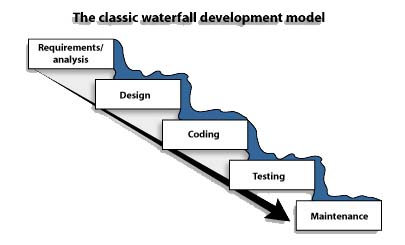
\includegraphics[scale=0.8]{waterfall.jpg}
    \caption{Waterfall model. You should see why it is called waterfall from this picture.}
    \label{Waterfall}
\end{figure}

\subsection{Prototyping}

Sometimes, you want to produce a product as soon as possible so you can conquer the market sooner. In that case, the waterfall approach is not gonna be very usefull. The prototyping process though, can help you towards this goal.\\

The idea is to produce some prototype as soon as possible, test it and then, iterate over it again and again until the final product is fully functionnal. It is a trial-and-error process. This works especially well when the final product requierements are not fully known. By presenting a prototype to the client, he is able to give feedbacks and explain the following most wanted features. Like for the waterfall model, we have a plan for the whole process:\\

The whole product is divided into as many sub-product as needed. Each of those division will be prototyped on top of the last ones until we get the final product.\\

\begin{itemize}

\item System requierements are defined in as much details as possible.
\item A first design is created.
\item The first prototype is created.
\item Client reviews the prototype.
\item Devellopers change the prototype accordingly.
\item We repeat those steps as many times as needed.
\item The final product is constructed based on the last prototype.

\end{itemize}

Using this model, the probability to deliver a product that does not meet the client requierements is very small as he can give a feedback throughout the whole developement process. But there are some drawbacks to that.\\

Focussing on small sub-problems/sub-features distracts the developers from conducting a good and in depth analysis. This is also due to the lack of fully specified requierements from the start. Adding more and more features on top of existing ones can quickly create a complicated product both difficult to maintain and improve.\\

\begin{figure}
    \centering
    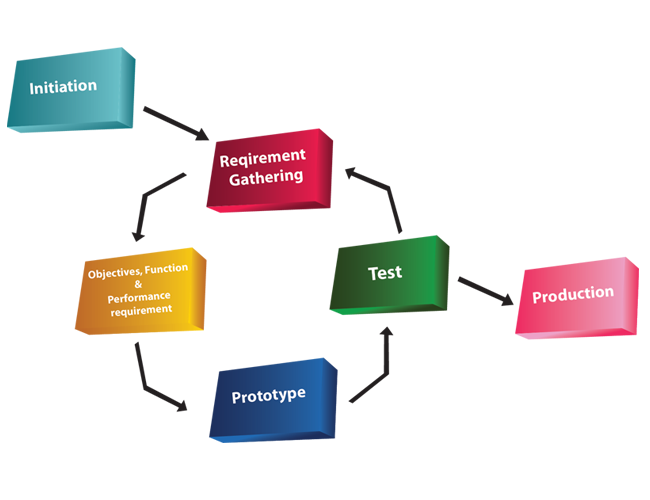
\includegraphics[scale=0.4]{prototyping.png}
    \caption{Schema of the prototyping process.}
    \label{Prototyping}
\end{figure}

\subsection{Agile}

Agile Software Development is based on twelve principles:

\begin{itemize}

\item Customer satisfaction by early and continuous delivery of valuable software
\item Welcome changing requirements, even in late development
\item Working software is delivered frequently (weeks rather than months)
\item Close, daily cooperation between business people and developers
\item Projects are built around motivated individuals, who should be trusted
\item Face-to-face conversation is the best form of communication (co-location)
\item Working software is the principal measure of progress
\item Sustainable development, able to maintain a constant pace
\item Continuous attention to technical excellence and good design
\item Simplicity—the art of maximizing the amount of work not done—is essential
\item Best architectures, requirements, and designs emerge from self-organizing teams
\item , the team reflects on how to become more effective, and adjusts accordingly

\end{itemize}

There exists many different frameworks that complies to those principles. One of the most comonly used is Scrum~\cite{ScrumAlliance:2017}. With this framework, we work using sprints. A sprint is the basic unit of development in Scrum. The team fixes the timeframe during which the sprint must be done and then, fixes the scope of work that needs to be done during a Sprint Planning event.\\

At the end of each day, the team holds a Daily Scrum to answer the following questions:

\begin{itemize}

\item What did i do ?
\item What will i do to meet the sprint goals ?
\item Is there anything that block the team progress ?

\end{itemize}

Finaly, at the end of the sprint period, the team holds a Sprint Retrospective to answer the following questions:

\begin{itemize}

\item What went well ?
\item What could be improved ?

\end{itemize}

This allows for a very dynamic development process in which no ones get stuck too long on innefective or impossible processes.

\begin{figure}
    \centering
    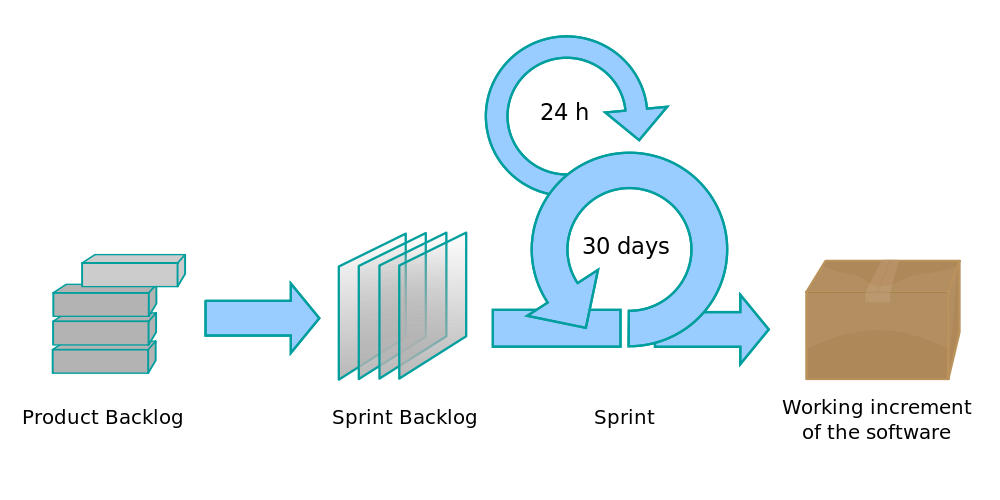
\includegraphics[scale=0.4]{scrum.png}
    \caption{Schema of the Scrum Framewrok. One of the most effective development process. This is only an example, the sprint duration is not always 30 days.}
    \label{Scrum}
\end{figure}

\subsection{Validation and verification}

Now that we have settled down our requirements specifications, we need to introduces the validation and verification topic. Validation and verification is what we use to make sure that our software is meeting the previously specified requirements. In short, that our software is exactly what we specified. Failing to this would produce a software that will maybe not meet the clients requirements and, therefore, be of little or no use to him.\\

Both concepts are closely related but are completely independant. Software validation is a procedure used to ensure that the software meets the user's needs and that the specifications were correct while software verification is a procedure used to ensure that the software follows the specified requirements~\cite{VnV:2016}. Following is a more formal definition:

\begin{itemize}

\item \textbf{Validation} is the confirmation by examination and through provision of objective evidence that the requirements for a specific intended use or application have been fulfilled~\cite{IEEEStd1990}
\item \textbf{Verification} is the confirmation by examination and through provision of objective evidence that specified requirements have been fulfilled~\cite{IEEEStd1990}

\end{itemize}

Simply put, validation is answering to "Are we trying to build the right thing ?" whil verification is answering to "Have we made what we were trying to make ?". Of course, in our case, we are more interested in the verification part and we will leave the validation part out of this work. We will assume that the requirements are correct and therefore that if we follow them, the built software will be the one our client wants.

\subsection{Code coverage}

Code coverage is a metrics used in software testing that basically tells you how much of your code has been tested. It can be computed on many differents criteria like how many subroutines have been called, how many line of code have been interpreted and so on.\\

The idea behind this metric usage is that, if all of your code is tested, then there is probably no bugs left, or at least, there is a good probability that we will encounter less bug in a completely tested software than in an untested one. Getting a good code coverage is therefore a key point in testing as it improve the software quality by reducing the probability of faults left in it~\cite{TestingForContinuousDelivery:2016}.

\subsection{Black-box and white-box testing}

Black-box testing and white-box are two terms used by softwares testers to describe how they approach their testing~\cite{Patton:2005}. They describes two of the most common used techniques in software testing.

With black-box testing, also known as functional testing, we consider the software as a black-box and we have no knowledge of what is inside of it nor on how it works. This is the opposite of white-box testing where the whole software is known from the inside, all the code is accessible and we have a deep knowledge of how it works.\\

Both of those approaches have their own advantages and drawbacks. In white-box testing, the tester is testing functionalities that are already developed and he can miss needed features that have been forgotten. He has a very good code coverage as he can produce test cases for every specific details by reading the code. White-box provides an internal perspective of the software.\\

Black-box testing, on the other hand, provides another point-of-view and does not requires a deep knowledges of the code to operate. Test cases are designed following the requirements and not the code itself so if all the tests are succesful and that all the requirements are entierly covered by the designed test, we have a proof that our software meets the requirements.\\

White-box testing is more or less done by developpers themselves while black-box testing can be performed by anyone with poor programing skills. Code coverage can not be used while doing black-box testing for the obvious reason that you dont know what is done internally so you dont know what part of the software code is interpreted.

\subsubsection{Grey-box testing}

There is also a third option there which is called "Grey-Box testing". We are doing Grey-Box testing when we do both Black-Box testing and White-Box testing.

\subsection{Static and Dynamic testing}

Two other terms used in software testing are static and dynamic testing. Static testing is the process of reviewing something that is not running. For example, some compilers (like gcc) perform static testing by finding unafected variables, unused variables, dead code, syntax errors and so on. Dynamic testing, on the other hand, is performed while the program is running.

\subsection{Type of testing}

There exists a lot of different types of software testing, explaining them all is way out of the boundaries of this work so we have choosen 6 of them that are closely related and can be spanned on a whole software devellopement process~\cite{Laurie.W:Black-box}.

\subsubsection{Unit testing}

Scope: White-box testing\\
Who: Coder\\

Unit testing is a software testing method by which individual units of source code, sets of one or more computer program modules together with associated control data, usage procedures, and operating procedures, are tested to determine whether they are fit for use. The goal is to isolate each part of the program and show that the individual parts are correct~\cite{AutomatedDefectPrevention:2007}.\\

In a more practical point-of-view, it's about isolating each function/method/class/... from the code and test their behavior for a wide range of input values. A lot of faults can stay undetected after this step. One of the reason of this being that people who write unit-test have a deep knowledge of the underlying code. This knowledge influence them when writing unit-test so it becomes really hard to set realistic test cases. Also, if those who write the unit-test are the same ones that wrote the code that is being tested, the test code is likely to be as faulty as the code being tested itself !

\subsubsection{Integration testing}

Scope: Black-box and white-box testing\\
Who: Coder\\

Integration testing is the phase in software testing in which individual software modules are combined and tested as a group. It occurs after unit testing and before validation testing. Integration testing takes as its input modules that have been unit tested, groups them in larger aggregates, applies tests defined in an integration test plan to those aggregates, and delivers as its output the integrated system ready for system testing~\cite{TestingInSoftwareDevelopment:1987}.

\subsubsection{Functional testing}

Scope: Black-box testing\\
Who: Independant tester\\

Functional testing is about testing each functionality of the whole system as described in the requirments.

Functional testing tests a slice of functionality of the whole system. Functional testing does not imply that you are testing a function/method of your module or class. If the functionalities wanted are:
\begin{enumerate}
\item Sending invoices to clients
\item Creating invoices
\item Adding clients
\end{enumerate}

Then you will have test cases that try to add clients, another one that try to send invoices and acknowledges that the client, preferably a fake one, received it and a last test case that will create various different invoices.

\subsubsection{System testing}

Scope: Black-box testing\\
Who: Independant tester\\

System testing involves putting the new program in many different environments to ensure the program works in typical customer environments with various versions and types of operating systems and/or applications~\cite{Laurie.W:Black-box}. System testing is testing conducted on a complete, integrated system to evaluate the
system compliance with its specified requirements~\cite{IEEEStd1990}.\\

This is especialy relevant in computer science where every computer is built from different component and can have many different operating systems. To perform system testing, you will usualy run the program on different operating systems (Unix based systems or DOS based systems) and also on different hardware configuration. Of course, testing every possible combination is not possible so some exotic systems can still prove themselves unable to run the program after this steps. Of course, if your program is built to run on a specific pre-defined system, this testing will be really straigthforward.

\subsubsection{Acceptance testing}

Scope: Black-box testing\\
Who: Client\\

Acceptance testing is formal testing conducted to determine whether or not a system satisfies its acceptance criteria (the criteria the system must satisfy to be accepted by a customer) and to enable the customer to determine whether or not to accept the system. More formally, the system is tested to verify that it meets the given specifications or contract.\\

Usually, the user will provide some test or use case for each desired functionality. You can add your own test to those but at least the client test must be statisfied before trying to deploy the product otherwise the client will probably not even try the product.

\subsubsection{Regression testing}

Scope: Black-box and white-box testing\\
Who: Coder\\

Regression testing is a type of software testing used to ensure that a software that was previously developed and tested still meets the previously defined requirments after a modification has been introduced into it such as a bug fixes or enhancements. The purpose is to make sure that the newly introduced modifications do not damage any previously-working functionality.\\

Practically speaking, we will only add new test when we are adding new functionalities and we will remove test only when the functionnality covered is no longer needed or maintained. Then, if all the tests are still running without error on our new software, we will assume that previously developed functionality still works.

\subsubsection{Beta testing}

Scope: Black-box testing\\
Who: Client\\

This step is performed when the software is fully or well developed. The software is shipped to a limited amount of users so that they can test it as they wish. The purpose is to detect fault by providing inputs that testers have not thought about because of their advanced knowledge of the software and its purpose.

\subsection{Requirements-based testing}

Requirements-based testing is a testing approach in which test cases, conditions and data are derived from requirements~\cite{IBMRequirementBasedTesting:2017}. Those test can be performed from the start of the development process and to the end of it~\cite{BenderRBTRequirementBasedTesting:2017}. Of course, if the requirements are not good, those test will be of little use. Good requirements are critical but requirements checking is, again, out of our scope. So we will simply assume that we have good requirements for this work.\\

Requirements-based testing is exactly what we are trying to do with black-box testing. For each given requirements stating, for example, that we want to produce some result Y when you give some input X, we want to produce a test case that maps the input X to our software and gets the output Y'. Comparing Y and Y' will allow us to decide whether or not, there is a fault and/or decide if the requirement is met or not. If not, our software is not built correctly and we need to work more on it before shipping it for the client.\\


%------------------------------------------------------------------------%
%                                                                        %
%                                                                        %
% MODEL CHECKING                                                         %
%                                                                        %
%                                                                        %
%------------------------------------------------------------------------%

\clearpage
\section{Formal Verification and Model Checking}

Our goal is to be able to verify that any kind of product, software or hardware, is working as expected. Formal verification can help us to achieve this goal. It is a process that allows us to check wether or not a given model satisfies given properties. You can, for example, create a model of a given software and verify that it does not contains bug. To be able to do that, both the model and the specification must be formaly described in a mathematical language. Let's introduce \gls{fsm} which is the generalization of every system's modeling.\\


%------------------------------------------------------------------------%
%                                                                        %
%                                                                        %
% FINITE AUTOMATA                                                        %
%                                                                        %
%                                                                        %
%------------------------------------------------------------------------%

\subsection{Finite State Machine}

A \gls{fsm} is a mathematical model of computation. It is a mathematical structure used to provide an abstract description of the behavior of a system. This mathematical structure is composed of a list of state. There is usualy a state for each possible 'state' of the system's memory and thus, we will only talk about finite state machine because the system we try to describe is made of finite memory and because of that, it can only have a finite set of state which is a function of it's internal memory.\\

For example, if we try to represent a system with only 8 bits of memory, we can only have $2^8 = 256$ states.\footnote{A bit or binary digit can only take one of two possible values often represented as $0$ and $1$.}

A \gls{fsm} can be in exactly one of a finite number of states at any given time. The FSM can change from one state to another in response to some external inputs. The function that maps state and inputs to states is called a transition. A FSM is defined by its list of states, its initial state, the input alphabet and a set of transitions~\cite{FSM:2017}.\\

The input alphabet is the list of every symbol it can receive in any given state. For example, an input alphabet could be a list of keyboard's key if we consider a \gls{fsm} that simulates the behavior of a text editor.The key points here are that you need to have a finite set of state and a finite set of transitions.\\

More formally speaking, a \gls{fsm} is a quintuple $(\Sigma, S, s_{0},\delta, F)$ where:

\begin{itemize}
\item $\Sigma$ is the input alphabet.
\item $S$ is the set of state.
\item $s_{0}$ is the initial.
\item $\delta$ is the state-transition function $\delta:S\times \Sigma \rightarrow S$.\footnote{This hold only for deterministic \gls{fsm}, we'll see later how to express $\delta$ for non-deterministic \gls{fsm} and what non-deterministic/deterministic \gls{fsm} means.}
\item $F$ is the set of final state.
\end{itemize}

To this, we need to apply the following rules:

\begin{itemize}
\item $\Sigma$ is a finite set
\item $s_{0}$ is included in $S$
\item $F$ is a subset of $S$ and can be empty
\end{itemize}

Because of those rules, a transition function can start and end in the same state, thus creating a loop on the state. $\delta$ is conventionaly allowed to be a partial function. This means that $\delta(s, e)$ does not needs to be defined for every possible combination of $s \in S$ and $e \in \Sigma$. This allows us to have a finite $\delta$ transition function even when the input alphabet $\Sigma$ is not finite or defined.\footnote{This is crucial for our practical case describe later on.}

About the input alphabet, we usualy define every input as a character or token read on the input tape of the \gls{fsm}. Where the input tape is a sequential list of every symbols feed into the system. This is a lot like a Turing Machine.

\subsubsection{Acceptors}

An acceptor takes a set of input from the input alphabet and run a \gls{fsm} on it. Every state of the acceptor is either and accept state or a reject state. When the computation ends in an accept state, we say that the input is accepted and the input is not accepted otherwise (figure~\ref{acceptor}). The set of sequence of input symbols accepted by an acceptor is called a regular language.\\

\begin{figure}
    \centering
    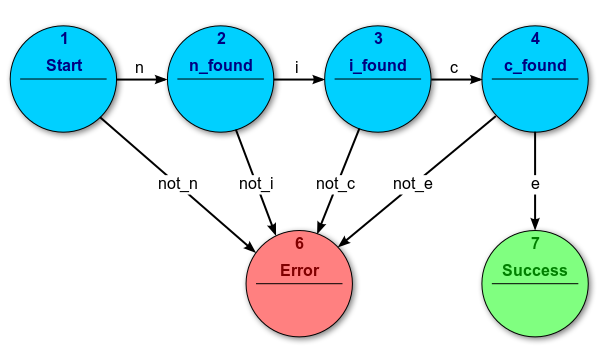
\includegraphics[scale=0.8]{acceptor.png}
    \caption{Example of acceptor for the string 'nice'~\cite{FSM:2017}}
    \label{acceptor}
\end{figure}

\subsubsection{Non-Determinism}

A \gls{nfa} is a kind of \gls{fsm} in which transition does not requires the reading of an input symbols. We can take transitions from one state to another without looking at the input tape. The decision of taking such a transition is done in a non-deterministic way. And some transition can also lead to more than one state. So reading a given symbol $x$ in state $q1$ can lead to $q2$ or $q3$ for example (see figure~\ref{nfa}).~\cite{FA-DecisionProblems:1959}

Formaly speaking, we represent a \gls{nfa} with a 5-tuple, $(Q, \Sigma, \Delta, q_0, F)$ where:

\begin{itemize}
\item $Q$ is the finite set of states
\item $\Sigma$ is the input alphabet
\item $\Delta$ is the transition-function $\Delta: Q \times \Sigma \rightarrow P(Q)$ where $P(Q)$ is the powerset of $Q$
\item $q_0$ is the initial state with $q_0 \in Q$
\item $F$ is the set of accepting states where $F \subseteq Q$
\end{itemize}

In a \gls{nfa}, the input alphabet $\Sigma$ usualy contains a special symbol for representing a transition that can be taken without reading the next input symbol on the tape. This symbol is $\epsilon$.\\

\begin{figure}
    \centering
    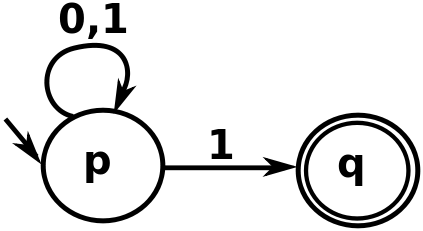
\includegraphics[scale=0.4]{graph/nfa.png}
    \caption{Example of a \gls{nfa}. In state $p$, reading the symbol $1$ can lead to $p$ or $q$~\cite{NFA:2017}}
    \label{nfa}
\end{figure}

It is well known that a \gls{dfa} is equivalent to a \gls{nfa}. One can translates from one to another quite easily. Thus this paradigm adds only a bit of freedom in the way we describe the automaton.\\

\subsubsection{Description of Finite State Machine using graphs}

Having a more human friendly way of presenting \gls{fsm} is possible using graphs. Any \gls{fsm} with a finite set of nodes and a finite $\delta$ transition function can be shown as a graph~\cite{Keller-FSM}.\\

To show a \gls{fsm} as a graph, we create a directed empty graph $G$. Then, we add a node for every state of our \gls{fsm} and we add an arrow for every transition defined in $\delta$ with the starting point being the current state and the endpoint is the goal of the transition. Finally, we add an arrow starting from nowhere and pointing to the node representing the initial state.\\

If we have accepting state in our \gls{fsm}, we represent the node for those state with a double circle. This gives us a graph we can display like in the figure~\ref{battcycle}. For comprehension sake, we have also labeled each node with a brief state name and every transition with an unique name based on the starting node.

\begin{figure}
    \centering
    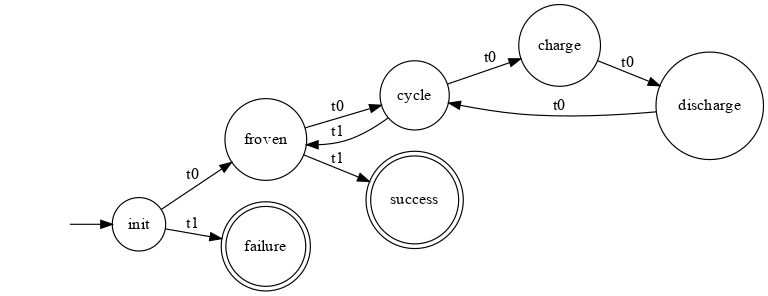
\includegraphics[scale=0.4]{graph/BatteryCycle.png}
    \caption{Example of a \gls{fsm} shown as a graph.}
    \label{battcycle}
\end{figure}

\subsubsection{Alternate Finite Automaton}

An \gls{afa} is a 6-tuple, $(S(\exists), S(\forall), \Sigma, \delta, P_0, F)$, where:

\begin{itemize}
\item $S(\exists)$ is a finite set of existential states
\item $S(\forall)$ is a finite set of universal states
\item $\Sigma$ is a finite set of input symbols
\item $\delta$ is a state-transition function $\delta: (S(\exists) \cup S(\forall)) \times (\Sigma \cup \{ \epsilon \}) \rightarrow 2^{S(\exists) \cup S(\forall)}$
\item $P_0$ is the initial state with $P_0 \in (S(\exists) \cup S(\forall))$
\item $F$ is the set of final state with $F \subseteq (S(\exists) \cup S(\forall))$
\end{itemize}

In an \gls{afa}, transition are more complex than those we encountered in traditional \gls{fsm}. The transition we are working with can lead to more than one state ! This is used to represent logical AND and OR with transitions (see figure~\ref{afa}).\\

\begin{figure}
    \centering
    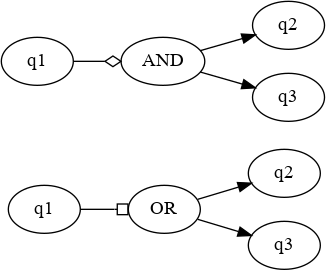
\includegraphics[scale=0.8]{graph/afa.png}
    \caption{Example of a \gls{afa}.}
    \label{afa}
\end{figure}

The introduction of those new transition type introduce a lot of complexity in the computation of the automaton. When we take an AND transition, we need to run a second automaton in parallel for each state the transition leads to and when we ecounter an OR transition, we behave like a non-deterministic automaton by taking one of the possibilities non-deterministicaly.\\

Thus the computation of such an automaton is now a tree. And deciding wether or not an \gls{afa} accepts a word $w$ if there exists a run tree on $w$ such that every path ends in an accepting state.~\cite{AFA:2017}\\

\subsubsection{Timed Finite State Machine}

Those are finite automaton with real-valued clocks added to it.~\cite{TimedAutomaton:2016} This allows us to do things like this:

\begin{itemize}
\item After 10 seconds, send this on inputs
\item After 5 seconds, read this on outputs, then wait 5 seconds and send this on inputs
\item Receive a data every 30 seconds or go to failure state.
\end{itemize}

The key point to describe timed automaton is that we now have clocks that can be used for transition. There are different kinds of timed automaton, the difference being the amount of used clocks and their scopes.\\

The most basic case is the one in which you can only use one clock with a global scope (all the automaton has access to it). You can reset the clock when you take a transition or in a given state. That's what we use in the figure~\ref{timed_automata_e1}.\\

\subsubsection{Markov model}

Markov Model is a stochastic model used to model randomly changing systems~\cite{1165342}~\cite{MarkovModel:2017}. The difference between a classic \gls{fsm} and a Markov Model is simply that the Markov Model take transitions randomly based on given probabilities.\\

This particular type of Markov Model is the simplest one. Probabilities are not influenced by previous state of the system. We will not introduce the other types of Markov Model here as we don't need them later on.

\begin{figure}
    \centering
    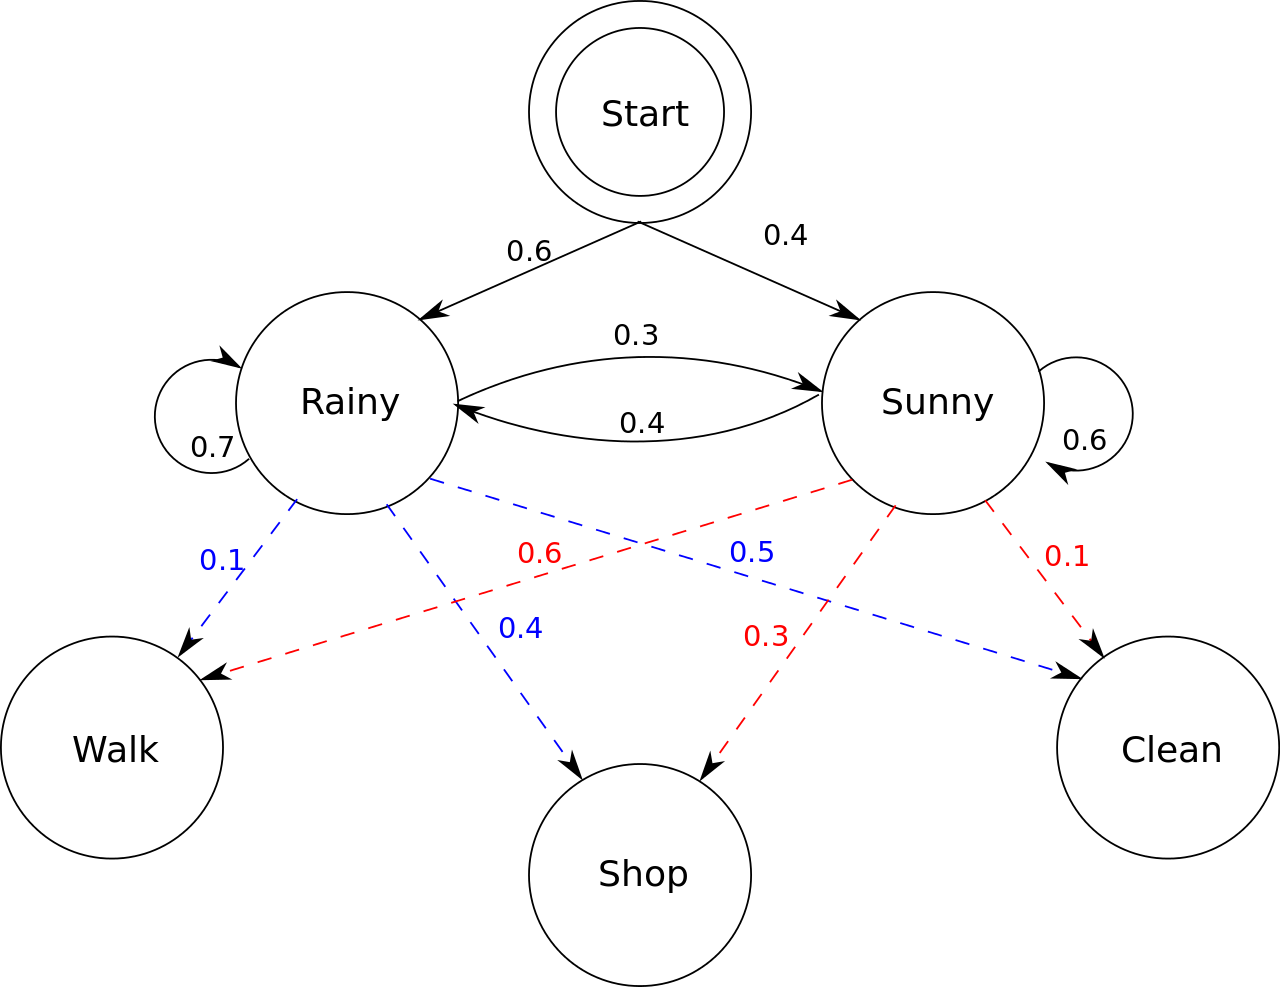
\includegraphics[scale=0.3]{MarkovModel.png}
    \caption{Example of a Markov Model. It shows the probabilities for the weather to be sunny or rainy and then, the probabilities for the person to go take a walk, clean or go shopping.}
    \label{MarkovModel}
\end{figure}

\subsubsection{Probabilistic Timed Automata}

Those kind of \gls{fsm} can be seen as Timed \gls{fsm} in which we added probabilistic transition like the ones used in a Markov Model.

\subsubsection{Others}

We can imagine a lot of other type of \gls{fsm}. For example, we discussed the possibility to mix timed automaton and alternate automaton. Such an automaton would need its own formal mathematical description and anylizis to make sure that it can succesfully be used to solve given problems.\\

The final choice we made is such a \gls{fsm} but we will describe it formally later on.

\subsection{Applications}

One of the first question one should ask is how is model checking and formal verification used in the everyday life or at least, for some projects. The following examples of what is currently used in this domain where taken from the most used tools at the time this paper was written. Unfortunately, this choice is rather subjective as metrics about each possible software usage is not always available but the only thing that interest us is to know how they works and what they have in common.

\subsubsection{UPPAL}

\begin{figure}
    \centering
    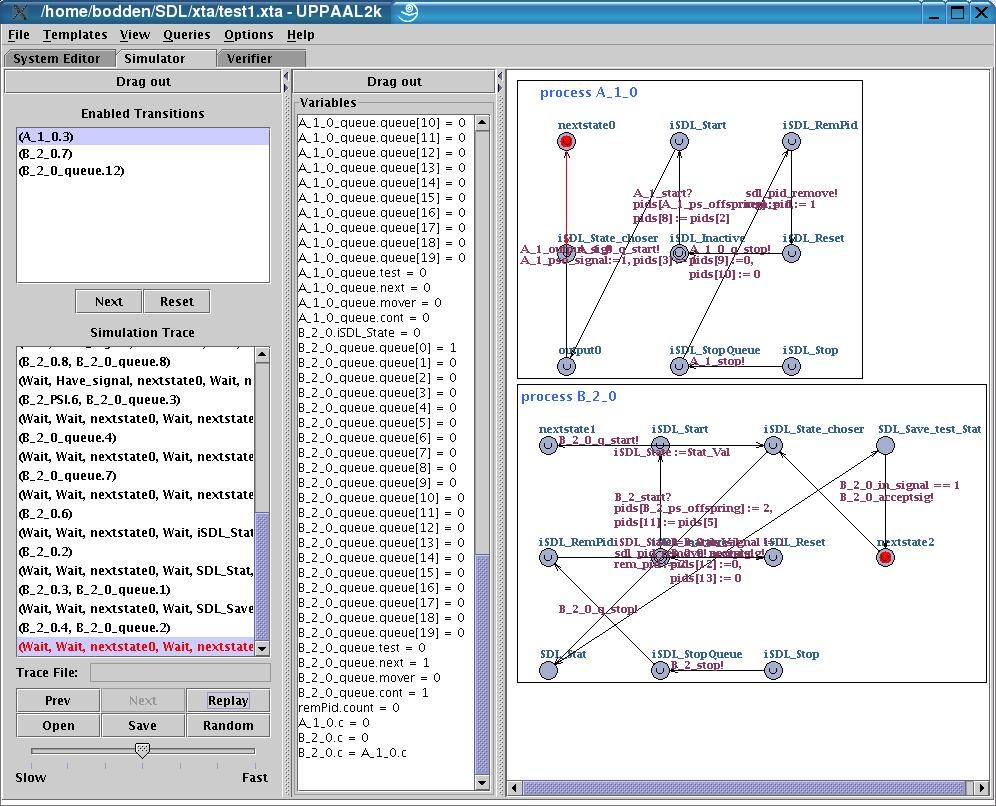
\includegraphics[scale=0.3]{UPPAAL_trace.jpg}
    \caption{Main window of UPPAAL for the simulation part. You can see the execution trace in the lower left corner of the window as well as the model of the system on the right, shown as a \gls{fsm}}
    \label{UPPAAL}
\end{figure}

The first software we came accross while searching for such applications was UPPAL. UPPAAL is a rather complete tool to work on model checking and formal verification. With it, one can modelize a system, simulate and verify it. All the three steps in only one tool~\cite{Bengtsson1996}~\cite{Behrmann2004}~\cite{Larsen1997}.\\

UPPAAL was a great source of inspiration for some features of our own tool. We where specificaly interested with the simulation tools wich allows to navigate through the execution steps and visualizing what is going on with the model of our system. Also, UPPAAL uses \gls{fsm} which conforted us in our choice of such tool.\\

\subsubsection{PRISM}

\begin{figure}
    \centering
    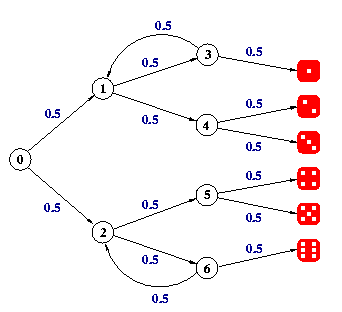
\includegraphics[scale=0.6]{PRISM_model.png}
    \caption{Example of model used by PRISM. This model was generated usign the lines of code in figure~\ref{PRISM_code}.}
    \label{PRISM_model}
\end{figure}

We where also interested by PRISM, which is a tool for modelization and verification of probabilistic systems. PRISM supports different kind of probabilistic models like \gls{dtmc}, \gls{mdp}, \gls{pa}, \gls{ctmc} and \gls{pta}.\footnote{Probabilistic Automata are Markov Chains that also supports deterministic transitions.}~\cite{Kwiatkowska2011}~\cite{Hinton2006}\\

PRISM uses a uniform modelling language for all the probabilistic models that it supports. This is a textual language, based on guarded command notation. See figure~\ref{PRISM_model}, this model was generated using the following lines of code:

\begin{figure}
    \label{PRISM_code}
    \begin{lstlisting}[frame=single,caption="Dice model in PRISM",label={lst:PRISM_code}]
dtmc

module die

    // local state
    s : [0..7] init 0;
    // value of the die
    d : [0..6] init 0;

    [] s=0 -> 0.5 : (s'=1) + 0.5 : (s'=2);
    [] s=1 -> 0.5 : (s'=3) + 0.5 : (s'=4);
    [] s=2 -> 0.5 : (s'=5) + 0.5 : (s'=6);
    [] s=3 -> 0.5 : (s'=1) + 0.5 : (s'=7) & (d'=1);
    [] s=4 -> 0.5 : (s'=7) & (d'=2) + 0.5 : (s'=7) & (d'=3);
    [] s=5 -> 0.5 : (s'=7) & (d'=4) + 0.5 : (s'=7) & (d'=5);
    [] s=6 -> 0.5 : (s'=2) + 0.5 : (s'=7) & (d'=6);
    [] s=7 -> (s'=7);

endmodule
    \end{lstlisting}
\end{figure}

Again, this tools uses \gls{fsm} to modelize different systems.

%------------------------------------------------------------------------%
%                                                                        %
%                                                                        %
% CASE STUDY                                                             %
%                                                                        %
%                                                                        %
%------------------------------------------------------------------------%

\clearpage
\part{Case study}

Now that you now what software testing and \gls{fsm} are all about, lets introduce the case that is of interest to us, namely, Nursery ! I'll first introduce the Railnova enterprise and the system we will work with all along this paper. Then I will explain why this work is of critical importance for them and generaly speaking, for every software development process.

\clearpage
\section{Railnova}

This work is done in partnership with Railnova. Railnova is a technology company that provides telematics and software solutions to the railway industry. Their headquarter is located in Brussels and they count approximatively 30 employees. Some of them coming from the ULB/VUB.\\

The main goal of this work is to develop a better testing suite for their embedded software called \gls{railsteros}. Of course, the developed solution will not be limited to a particullar software and our scope is a lot wider than that.\\

\subsection{Existing system}

\gls{railsteros} is a software developed at Railnova which purpose is to collect and stream data from a train to a server. This data is then processed to give various insigths about the train status. Thus allowing Railnova's client to manage their fleet with ease.\\

The \gls{railsteros} is executed on a dedicated hardware also built by Railnova which is called \gls{rug}. Those \gls{rug} are mainly installed in trains in Germany, France, Belgium, Netherlands and Spain at the time this work was written. More specifically, the \gls{rug} is installed in the engine of trains.\\

This dedicated hardware provides a lot of data from the train. We can access informations like remaining fuel (if it is not an electrical engine), the total running time since last power on of the engine, where is the engine located, current speed if the engine is moving and all the data that the client wants to access remotely.\\

Every engine is more or less unique. They can use a wide range of different component and thus have different parameters like their maximal speed when loaded or not, the maximal weigth they can carry or even the number of wheels the engine uses. Because of that \gls{railsteros} need to accept a wide range of different configuration so we don't stream fuel remaining if we are on an electrical engine for example. We can also have two kinds of motors that give information about their speed without using the same type of cable or protocol. To achieve this flexibility, we allow \gls{railsteros} to start only a subset of its internal software using some configuration files. All this software's modules, which we call \gls{daemons}, are small applications used to interface with a given protocol. For example, we have one deamon that is dedicated to GPS location's informations. The set of deamon we use, which is defined in the configuration files, defines what type of engine we can handle and what operations we can do.\\

To retrieve all those informations, we need to use different communication protocols and wires because engines built by different companies will have different behaviors and communication protocols. All of them, we will call interfaces. Each of those interface needs proper test that relies on the used protocol, we want to be able to describe our needs by saying things like "I want this particular data when I receive this kind of message on this interface". As there is a lot of them, this will take time to implement proper testing for all of them so we will only cover a subset of them in this paper but we will provide a generic way of implementing test for them all.

\subsection{Railster Universal Gateway}

As stated before, \gls{railsteros} is running on \gls{rug}. Those hardware are built by Railnova. Actually, the majority of them are in their first version (RUG1) but the RUG2 is on its way. It is important to keep that in mind to understand why we tried to keep this work as generic as possible. Indeed, in a year, maybe less, the majority of the product used will be RUG2 so if the system can only work for a dedicated and specific hardware, we will need to start over all this work for the RUG2.\\

\gls{railsteros} is being develloped incrementally since the start of the company. It means that the software is kind of messy with all the new features coming in and the old ones being deprecated or deleted. Actualy, there is more than 10 different versions of the software in production and those are not the only exisiting versions.\\

It is frequent to encounter new bug after the release of a new version that were supposed to be fixed since earlier versions simply because the new changes re-introduced the problem. This is mainly because Railnova is a young company, a start-up, and the work priority are realy end-user scheduled. If a system stop working, a quick fix is developed and pushed to production as fast as possible to avoid loosing too much money but the cost on the long run for this operation can be greater than what we saved by fixing the problem quickly.\\

Say that the problem is fixed by a quick and dirty patch. Then, one year later maybe, a major problem arise because all the fixes deployed are preventing us from adding wanted features. Then, the whole system is to be re-developed from the start. That was what hapenned when they tried to put \gls{railsteros} on the RUG2. RUG1 was developed the quick and dirty way to be on the market as soon as possible. So a lot of concepton errors were made. The software had been modified to a point where it needed all those conception errors from the RUG1 to operate correctly.\\

\subsection{Short story}

Some of the \gls{rug} were experiencing troubleshoot during then end of fall 2016. 8\% of the fleet had to be replaced by the team for unknown reasons. After a bit of testing, some members of the team thought that it could come from an unexpected electrical over-consumption of the \gls{rug} while connecting to a GPS antenna. To validate this hypothesis, some testing had to be done. It was the end of summer so the outside temperature was going down so the team thought that maybe it had something to do with that.

The test procedure was defined as follow:
In a thermic chamber set to a temperature of -10 celsius degrees, to simulate the outside temperature as best as we can, we put a \gls{rug} and we connect with a computer next to it to the serial communication port of the system. Once we are connected, we issue some command to mannualy choose which GPS protocol to use out of the four of them supported and for each of them, we manually set the emiting power of the GPRS chip in order to reproduce the problem seen on the practical field.\\

Those test were made, approximately 30 for different temperatures of the thermic chamber, different band and different emiting power. Those took one person an entire day of work ! That's because the thermic chamber needs an hour to set a fixed temperature, the system needs 5 minutes to reboot when we set the band to use and we wait 10 minutes for each test to be sure the problem did not appear (or did). After each test, if we want to do another one, we need to wait for the system to cool down as each time we boot it up, it produces heat.\\

And those tests are just to prove the initial hypothesis. Once this was proved, we wanted to know for sure, what emiting power we could use for each \gls{rug} (not only for one) depending on the band used and the external temperature. This would need hundreds of tests if not a thousand on a lot more than just one \gls{rug} to be able to make enough data and say for sure which levels are safe, which levels are risky and which levels are forbidden to avoid problems in the real world.\\

And that's without mentionning that the thermic chamber makes a lot of noise to work, wasting an entire room as people can not work long in such a noisy environment.\\

This is where the Nursery project comes in handy. The goal of it is to provide an environnement fully automatized to realize all those testing when we want, like during the night so the room stays silent during the day for men to work in, without needing one or more persons to take weeks or years of works.

\section{The economics of software testing}

Usually, when you work on a development project, you have many different development stages. The main ones are the proper development of the product and the final stage of the product, when it is shipped to the production environment.\\

Shipping the product to production simply means that you put the product into its real environment. In other words, you begin to manipulates real world data and not the tests sets that you where probably using during the development. In our case, we install a RUG running \gls{railsteros} in some engine.\\

But if the shipped product contains faults, it will probably begins to produce incorrect results and, depending on the product, it can even harm people or destroy things by using them incorrectly. The client will not be able to use the product he paid for to its full capabilities and will maybe want to switch to another company that produce more reliable products. Its easy to imagine other cases in which having fault in the final product must imperatively be avoided.\\

All of this comes with a cost, for example, we can imagine that we are working on a assembly line controller. If our controller (product) does not work correctly, the assembly line can be damaged because of incorrect usage or the materials being manipulated can be damaged too resulting in repair cost for the assembly line and incorrect/damaged product assembled that cannot be sold afterwards.\\

In the \gls{rug} ecosystem, if our product, \gls{railsteros} isn't working well, the \gls{rug} its running on will not send the intended data to the client. For him, it is like the engine itself is misfunctionning or not functionning at all if we are unable to send any data ! He will then need to send a team to the engine to find the problems and a lot of work will be delayed because the engine is not running and, of course, every step in this process is very costly for the client and for the company itself because when a product in production is faulty, we also need to get back the devices that are malfunctionning and, perhaps, every other device running the same software of having the same hardware. And finally, we need to replace them and invest time in correcting them or, at least, solving the issue for the other product versions.\\

\begin{figure}
    \centering
    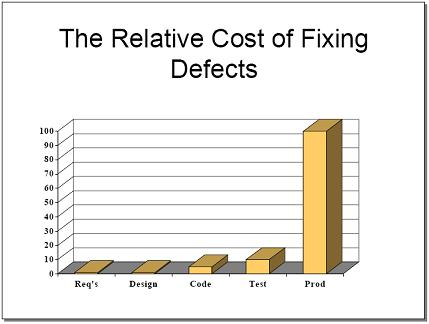
\includegraphics[scale=0.8]{STBC-costfixs.jpg}
    \caption{Relative costs of fixing faults~\cite{EconomicsSTBC:2017}}
    \label{STBC-costfixs}
\end{figure}

It is commonly believed that the earliest a fault is found, the cheaper it is to correct it~\cite{EconomicsSTBC:2017}~\cite{EconomicsWiki:2017}. The case we mentionned is the latest possible time to detect a fault so, according to the previous statement, it is also the costier ! Those reasons are why we want to create some process that can be used to drastically reduces the amount of unexpected faults in the final product. That's the main motivation behind the project that is the subject of this paper called Nursery.\\


%------------------------------------------------------------------------%
%                                                                        %
%                                                                        %
% CONTRIBUTION                                                           %
%                                                                        %
%                                                                        %
%------------------------------------------------------------------------%

\clearpage
\part{Contribution}

All the problems described above provides us a lot of informations. We know what can go wrong, we know what we need and we know that a proper validation of all the developed product is a key for success of any given product on the long run. So having a global view of what software testing is and what is the concrete problem we are dealing with, we will try to design a testing process that can be applied to it and possibly ot any other given problem that needs black-box testing. One of our main goal is also to design a tool that will be usefull and easy to use but we want it to be powerfull enough to be able to handle every test case we can think of.\\

\clearpage
\section{Requirements analysis}

So one of the problem that we are focussing on is what do we need to build a reliable process that can reduce drastically the odds of shipping incorrect or faulty products to our clients ?\\

To reply to this question, we need to analyze what we need or what are our requierments. We can begin by saying that we need to handle a set of inputs and a set of outputs. We also need rules to parse the set of outputs and validate them or not.\\

What we mean by saying "validating the outputs" is simply determining if those are the expected outputs or the correct outputs. If not, we encountered some invalid outputs meaning that our product is faulty and cannot be shipped.\\

For the \gls{rug}, we have a really huge amount of different inputs sources and all of them can produce a wide range of various outputs. So, for this work to be done in time, we choose to only cover a given subset of those inputs/outputs. But, we cover them, we'll try to give some general ways of handling them so this work can easilly be extended to all kind of inputs/outputs regardless of the project being considered.


\section{Testing environment}

The testing environment should emulate perfectly any given train/engine. Each train have a set of interfaces that are plugged into the tested system. What we mean by "interface" is one particular input type, those will be described later on. The system that will emulate the train (or the testing environment) will be given a set of "scenario"\\

Those scenario will describe what can happen to the system and how it will react to it. A strong constraint in the case that concerns us is that, those scenario will be writted by people with poor or no knowledge of advanced programming so we need to provide a simple yet powerful language to write those stories.\\

We will assume that our testing environment have a way of sending every kind of inputs to the software being tested and retrieved every kind of outputs from it. Of course, in some case this is very difficult to achieve. Lets consider a practical example that is happening for the \gls{rug} case.\\

The \gls{railsteros} communicates with a GPS/GSM chipset that is connected to antenna that are not under our control. This is an issue because under those circunstances, if the antenna can behave differently in production than during our tests sessions so some faults can goes undiscovered until that.\\

Some solutions exists for this kind of problems like having our own antenna or using development boards for this chipset. We could also try to write some kind of simulator that will interface with the GPS/GSM chipset but we would need to reverse engineer the whole GSM/GPS networks or at least one particular anenna which would be really time and ressource consuming. Not to mention that it will also probably be way costier than fixing hypotetical faults when they arise in the production envrionment. So the complex interfaces needed for those kind of technical component and specificaly, their implementations are not a simple matter and are way beyond the scope of this paper so we will not talk more about them. \\

In this paper and for case like this one, we will simply consider that it is not a part of the system that we can test. So every component that are part of the whole system being tested are provided with some interface that allows us to communicate with them, sends and retrieves data.\\

With that in mind, we want to be able to describe what happens on the input side of the studied system and then, what are the expected results or outputs produced. For example, when you put some money in a vending machine to buy a soda, the system is the vending machine, you don't know how it works (or at least, most people dont), you feed it some inputs (some money) and you expect a given output (a soda) (figure~\ref{vm-io}). This is exactly what you want to describe in your tests.\\

\begin{figure}
    \centering
    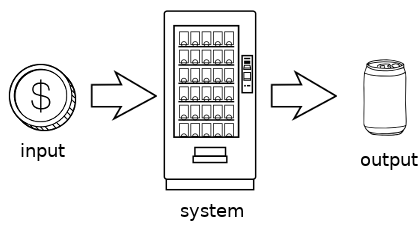
\includegraphics[scale=0.8]{vending-io.png}
    \caption{The vending machine I/O mapping}
    \label{vm-io}
\end{figure}

A naïve idea to do so could be to write a file mapping every possible inputs to every possible outputs and claim that our process works only when no unpredicted input/output pair occurs during some run of it (figure~\ref{io_map1}). But then, what if we want to produce a different output depending on how many times we seen some given output ? With this first idea, it would not be possible to handle this as we dont keep track the current state of the process. We don't have a way of counting how many given inputs have been encountered since the start of the process.\\

\begin{figure}
    \centering
    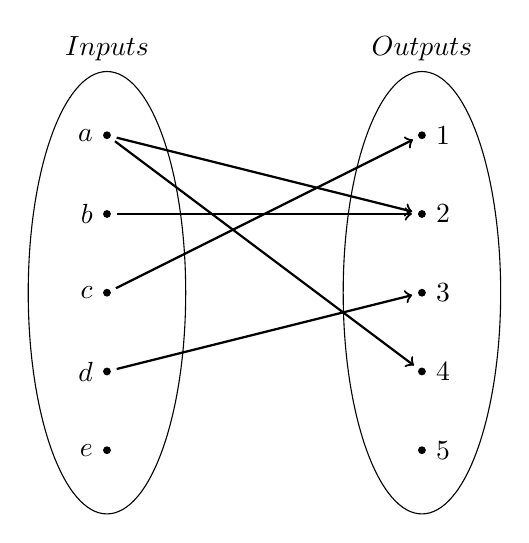
\begin{tikzpicture}[ele/.style={fill=black,circle,minimum width=.8pt,inner sep=1pt},every fit/.style={ellipse,draw,inner sep=-2pt}]
    \node[ele,label=left:$a$] (a1) at (0,5) {};
    \node[ele,label=left:$b$] (a2) at (0,4) {};
    \node[ele,label=left:$c$] (a3) at (0,3) {};
    \node[ele,label=left:$d$] (a4) at (0,2) {};
    \node[ele,label=left:$e$] (a5) at (0,1) {};

    \node[ele,,label=right:$1$] (b1) at (4,5) {};
    \node[ele,,label=right:$2$] (b2) at (4,4) {};
    \node[ele,,label=right:$3$] (b3) at (4,3) {};
    \node[ele,,label=right:$4$] (b4) at (4,2) {};
    \node[ele,,label=right:$5$] (b5) at (4,1) {};

    \node[draw,fit= (a1) (a2) (a3) (a4) (a5), minimum width=2cm, label=above:$Inputs$] {} ;
    \node[draw,fit= (b1) (b2) (b3) (b4) (b5), minimum width=2cm, label=above:$Outputs$] {} ;
    \draw[->,thick,shorten <=2pt,shorten >=2pt] (a1) -- (b4);
    \draw[->,thick,shorten <=2pt,shorten >=2pt] (a1) -- (b2);
    \draw[->,thick,shorten <=2pt,shorten >=2] (a2) -- (b2);
    \draw[->,thick,shorten <=2pt,shorten >=2] (a3) -- (b1);
    \draw[->,thick,shorten <=2pt,shorten >=2] (a4) -- (b3);
    \end{tikzpicture}

    \caption{Not explicit schematisation of a valid mapping of inputs to outputs, all possible cases are not taken into account. On the left, the input we send into the system and on the rigth, the outputs we can receive. Arrows shows what are the expected outputs for a particular input}
    \label{io_map1}
\end{figure}

This first idea gave us an important lesson, we need to keep track of the state of the process or at least of what hapenned before the current time. This does correspond to what we call \gls{fsm} and this is why we introduced them earlier.\\

\section{Choices}

When asked what is the type of \gls{fsm} that fits our needs the best, we want to give the best possible answer. To do that, we need to rank the different possibilities that we have introduced based on the following criteria. First, we want to make sure that a particular \gls{fsm} type is possible to apply in our case. If it is an abstract \gls{fsm} that uses infinite memory or another paradigms that is impossible to implement on modern computer, we know that we can discard it.\\

Then, how easy it is to describe a system's behavior with such \gls{fsm} ? If it takes to much times or if we find it too difficult for non-technical peoples to describe a system's behavior using that particulare \gls{fsm} type, we know that it will probably be deprecated over time and wont be used as it should be.\\

Lastly, if the choosen \gls{fsm} introduces restriction on what can be described, those restriction must not prevent us from doing every testing needed. And if it introduces new possibilities that allows us to describe more system's behaviors, the complexity that it introduces into the system should be worth it.\\

Those three criteria are the ones that where choosen as the most relevant for the choice of the \gls{fsm} that will be used.

\begin{itemize}
\item Is it possible to implement ?
\item Is it user friendly ?
\item Does this introduces restrictions ?
\end{itemize}

Lets review the possible choices we have and justify the one we picked. But first, let's explain what are the main differences between our practical case and theory. In theorical \gls{fsm}, the number of state is upper bound by the system's internal memory. If we want to test every possible state it would gives us $2^x$ states to analyze (where $x$ is the system's internal memory expressed in bit). In modern computers, this memory can be around two to height gigabits maybe and this is raising every passing years. So having to describe what should happen in $2^2*10^9$ different states is not really a possible choice.\\

To address this problem, we need to abstract the state definition. We'll aggregate formal states into a more complex structure that we will still call a state but for the user, it will just be something like "initialisation state", "error state", "processing data state" and so on. A state will simply be a set of computation that needs to be applied. Three optional function, one for the computation needed when we reach the state, one for when we leave the state and the last one for the computation we need to do every time a new symbol is read.\\

The input alphabet $\Sigma$ formally defined earlier is also problematic, how can you describe every input received by a modern computer ? That requires very low-level knowledge and a lot of work. We want the user to be able to describe every states and transition without minding the $\Sigma$ input alphabet. To achieve this, lets define $\Sigma$ as a set of abstract inputs instead of character's set or token's set.\\

Now to the choice of \gls{fsm} model, why don't we simply pick the most simple case of \gls{fsm} ? The reasons are very simple, take this case: You want to be able to detect a failure that happen if you receive a given data more than 10 seconds after some given data. How can you do this ? Or even simpler, you want to detect a failure if you didn't receive any data for 30 seconds.\\

All of those case requires you to create a new input type that will be the time. Say you receive this input each time a second pass. Already, it is a lot like timed state machine but lets say we want to use a pure \gls{fsm}. Now, we need to add state for each seconds passed, so if we want to wait 30 seconds, we need 30 states with 30 transitions for each seconds and 30 transitions for the event of "a data has been received" that will go back to initial state. And all of this needs to be written by someone. You can easilly see why this is unpracticable. So clearly, in this case, \gls{fsm} are too limited if we want to handle this in a simple and practicable way.\\

Now with the \gls{afa}, the complexity of implementation required by this paradigm is quite important, we need to run multiple automaton, construct trees and analyze them. Compared to a simple \gls{fsm} implemnetation, this is quite a lot of work. So is it worht it ? To answer this question, we need to find practical case where such a paradigm would become indispensable and such case should be realy difficult to implement into a classic \gls{fsm} to justify choosing \gls{afa} as our main choice for the implementation of Nursery.\\

TODO Chandra and Fellah, Jürgensen and Yu construction $2^n$ states for non-deterministic and $2^{2^n}$ for worst case.\\

This left us with timed automaton. This is the choice we made. Those \gls{fsm} are really well adapted for our use case. Being able to manipulate time directly in our transitions and state gives us a lot of ease to write the code and its also very powerfull too ! With it, we are able, for example, to send a lot of data with a variable interval between them and then receive data accordingly. You can also decide to create a clock for timeout that will be reseted each time you receive a given data. There are really a lot of use case and some more will be described later on.\\

This choice of tool is also motivated by the fact that writting and understanding automaton is a very easy process. Designing a \gls{ui} to create automata and generating valid scenario out of it is a relatively easy process so this could be a way to meet the strong requirement that our solution shall be easy to use for not seasonned programmers.\\

As an example, take the pseudo-code showing how test are designed using this tool in listing~\ref{lst:python-pseudo-tsm}. We create 4 states, one, "init", is purely optional, it's purpose is for initializing external tools or some variables if we need them. Then a state that will simply do nothing, waiting for some data to arrive. A success and a failure state. This test works by looping in wait-state every time a data is received. The test success when enough time has elpased without any timeout and it fails at the first timeout encountered.\\

As we modified a lot the \gls{fsm} principles, we'll say that our \gls{fsm} succeed or fails when the test passed or failed. We will not say that our test accepts nor recognizes as we think this is not applicable for our case.

\begin{figure}
    \label{python-pseudo-tsm}
    \begin{lstlisting}[frame=single,caption="Pseudo test case example",label={lst:python-pseudo-tsm}]
class MyTest:
    add_state("init", enter=init_all)
    add_state("wait")
    add_state("success")
    add_state("failure")

    init.add_transition("wait", True)
    wait.add_transition("success", no_failure_since_long)
    wait.add_transition("failure", timeout)

    set_initial_state("init")

    listen_to("distant_data")
    \end{lstlisting}
\end{figure}

\begin{figure}
    \centering
    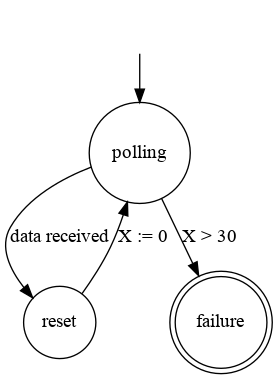
\includegraphics[scale=0.8]{timed_automata.png}
    \caption{Example of a timed-out timed automata. X being one of the clocks that can be used}
    \label{timed_automata_e1}
\end{figure}

\section{Mathematical description of our custom \gls{fsm}}

Theres a lot of modifications we did to the basic concept of \gls{fsm}. First of all, our input alphabet is never quantified. We don't know if it's finite or not. Theorically, we accept analogic inputs so it can be infinite but as we are working with computer, we know it will not be inifinite. The most important thing is that we don't need to quantify it to design our test, the choices we made keeps us from being forced to enumerate one and every possible input. Like we said, it will define itself based on what transition are defined in $\delta$ and a special symbol for a time step, let's say $t$.\\

Also concerning the states, they are not simple maping of the system's internal memory state. They are more complex abstraction of an arbitrary user defined state. And finaly, our $\delta$ transition function is allowed to be partialy defined, every undefined transition will have no consequences on the \gls{fsm} computation.


%------------------------------------------------------------------------%
%                                                                        %
%                                                                        %
% RESULTS                                                                %
%                                                                        %
%                                                                        %
%------------------------------------------------------------------------%

\clearpage
\part{Results}

This part is a in depth description of how the implemented system works, how it has been developed and what it can and cannot do. This is a more technical part dedicated to the implementation where we will not talk a lot about the mathematical concept behind it as those have already been explained before.\\

\clearpage
\section{Nursery}
\subsection{Architecture}
\subsection{Configuration}
\subsection{Command line tools}
\subsection{Web-administration}

%------------------------------------------------------------------------%
%                                                                        %
%                                                                        %
% CONCLUSION                                                             %
%                                                                        %
%                                                                        %
%------------------------------------------------------------------------%

\clearpage
\part{Conclusion}

This conclude my work at Railnova.


%------------------------------------------------------------------------%
%                                                                        %
%                                                                        %
%                                                                        %
%                                                                        %
%                                                                        %
%                                                                        %
%                                                                        %
%                                                                        %
%                                                                        %
% APPENDIX                                                               %
%                                                                        %
%                                                                        %
%                                                                        %
%                                                                        %
%                                                                        %
%                                                                        %
%                                                                        %
%                                                                        %
%                                                                        %
%------------------------------------------------------------------------%

\appendix

%------------------------------------------------------------------------%
%                                                                        %
%                                                                        %
% IO ABSTRACT                                                            %
%                                                                        %
%                                                                        %
%------------------------------------------------------------------------%

\clearpage
\section{Abstraction of Inputs/Outputs}

This part of the work is dedicated on describing how we managed to write simple piece of software that assure the link between Nursery and the real world/\gls{rug}.

\subsection{About Inputs/Outputs}

As we are working with a system that we feed with inputs and as we are ourselves feeded by the system's outputs, the concept of \gls{io} is a bit confusing. On the figure~\ref{io_abstract}, you can visually see why it is ambigous. So at this point, we'll simply consider that when we talk about inputs, we mean inputs of the system and when we talk about outputs, we talk of what the system produce.\\

\begin{figure}
    \centering
    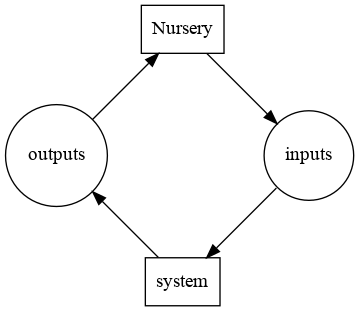
\includegraphics[scale=0.6]{io_abstract.png}
    \caption{Inputs of the system are outputs of Nursery and vice/versa}
    \label{io_abstract}
\end{figure}

\subsection{Outputs}

Let us start with the outputs. By outputs we mean all the data produced by the \gls{rug} or, more generally speaking, all data produced by the reviewed system. Those have been abstracted with a layer of object called output providers. Their goal is to retrieve outputs from various places and feed them into Nursery as they go.\\

For example, we can imagine that we want to receive some data each time the system sends data to a server, each time the system produce a sound, ect. All of this is possible as we simply need to write a script that detects that and use some kind of API to feed them througth Nursery.\\

\subsubsection{How does it works}

So, internally, each output provider defines a type of data it provides. For example, lets say we want to send data to nursery each time someone put a message on Twitter, we could name our data type: "TWITTER". Then, each test that is interested in data of type "TWITTER" will be subscribed to our output provider. It also allows us to ignore output providers for which no test are interested in. Practilly speaking, the only output providers rnning for a given test will be those that provide a data type usefull for the test.\\

Our provider is bundled with a mean of communication with all scenario that are subscribed to the data type it provide. With it, we can send data to every listenner with one simple call. All the communication process is managed internally in Nursery.
In our provider, we have a function that allows us to broadcast data to all listener. With this approach, we can write output providers for any type of data we can think of, all we have to do is defining the data type we provide and wich output provider provides it in a configuration file and then implement this output provider, that's it, now any scenario can listen to this particular data type.\\

One limitation though is that every data type can be produced by at most one output provider. On the other hand, every output provider can produce as much data type we want if this becomes a requirement at some point.\\

\subsubsection{Wanesy}

The first data type we have devellop is the WANESY data type. Data of type WANESY are triggered when we receive a new paquet of data sent by \gls{railsteros} to our server online. The method to retrieve them is simply to poll a JSON generated list of message by HTTP and check timestamp of generated messages, when a newer timestamp appears, we get the message and send it into Nursery.\\

Another more effective way of doing this would be by direct connection to the database but this would probably introduce security issues and is not really required for our use case. Note that it is still feasible in future version of this work.

\subsubsection{Log}
\label{subsec:log}

This data type is more of Grey-Box testing as it requires a direct serial connection into the studied system so we assume that we  are working on some kind of \gls{rug} andthat we know where the log are located on it. Nevertheless, this data type ("LOG") is usefull to provide more complex information wen fault arise and also help us to design more intrusive tests.\\

So even if they are a bit out of scope here, they do not invalidate the fact that our system can work on Black-Box testing.\\

To design those test, as we previously stated, we simply initiate a serial connection over the \gls{rug} and then download the file located in the log folder. Then, our script process it and send new lines into Nursery.

\subsubsection{Miscelaneous}
\label{subsec:misc}

As we talked in sub-section ~\ref{subsec:log}, we can initiate a serial communication with the \gls{rug}. Using this serial communication, we cand send command to it in an Unix environment so it's easy for us to check a lot of properties for our tests needs. Of course, this is clearly white-box testing, we know how the system is supposed to work so we can ask it if some key file are in place, if all environement variables seems to be correct, do some statistics on some values to be sure they have correct values all along our tests and things like that.\\

\subsection{Inputs}

Some of our test make use of external devices to produces inputs that are feeded to the \gls{rug} or to the hardware being tested. Those devices are, for example, an alimentation module that can charge the battery of our \gls{rug}, thermic chamber that can manipulate the current temperature to stress test our hardware in extreme conditions and things like that.\\

We also have more direct inputs like the ethernet connection, we want to be able to disconnect or re-connect the tested process or hardware.

\subsubsection{Alimentation}

\begin{figure}
    \centering
    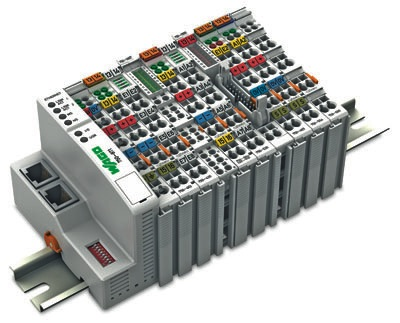
\includegraphics[scale=0.6]{wago_module}
    \caption{Module used to control the alimentation of a \gls{rug}}
    \label{wago}
\end{figure}

To control the alimentation, we need to send a command to a Wago module like the one of the figure~\ref{wago}. Those modules are connected via an ethernet connection thus we need to open a TCP port to communicate with it and then send a command to select which alimentation we want to control and what we want to do (power on or power off).

\subsubsection{Connectivity}

Controlling the connectivity is not something we did but this is easilly done by using some advanced switch. We simply need to communicate with it and send commands to deactivate the ethernet port to which the \gls{rug} is connected.

\subsection{The generic way}

Some techniques we mentionned, like in sub-section ~\ref{subsec:log} and sub-section ~\ref{subsec:misc}, use some kind of white-box testing. As one could expect, those techniques can only be used for one given device. We cannot initiate a serial connection with every process or hardware we want and all of them don't have the same Unix environment to dialog with.\\

But even the ones that applies to black-box testing can only be sepcific to some restraint set of process or hardware. Here, our techniques are all specific for \gls{rug} hardware. So every time we need to test a new kind of process or hardware, we will need to write some code to retrieve outputs and provides inputs for it. That's what we kept in mind all along this project by designing what we called \gls{op}.\\

\subsubsection{Outputs}

\gls{op} were designed to provides asynchronous capabilities to our tests. Polling \gls{io} is a process that takes a lot of times compared to the execution time of our test. With \gls{op}, we get the data when they are ready and we don't have to wait for them by freezing all the test. Two ways of retrieving data were implemented.\\

The most trivial way is simply to send data periodically to all test that needs it. The test knows he will receive data but he does not knows when. The test must be designed accordingly. This is usefull to fetch data that are not fixed like a speed, the current time or the remaining fuel for example.\\

The second way is to ask for data from the test. The call is asynchronous so you simply notify the \gls{op} that you are ready to receive some data or that you want it to fetch some data rigth now. This allows us to ask for one-time data like a serial number or other kind of data that are not supposed to change depending on the time.\\

So the first method is more for data you want to be able to monitor and the secnd method is more for data you will only need once.\\

\subsubsection{Inputs}

For inputs, we simply need some software to which we can send commands so we don't need so much abstraction as for the outputs. We are not in an asynchronous system. The way to go we adopted was simply to devellop some software that accepts command and send inputs to whatever we want.\\

One example was a software we used that can control a thermic chamber. With it, we were able to control the temperature in which our \gls{rug} was evolving. And of course, we can use it for other systems too, and we did it to test other pieces of hardware.

Another example, more specific, was a software used to control a device that could apply different electric loads to any device we connected with it. This was usefull for some hardware test that had nothing to do with the \gls{rug}.


%------------------------------------------------------------------------%
%                                                                        %
%                                                                        %
% TEST CASES                                                             %
%                                                                        %
%                                                                        %
%------------------------------------------------------------------------%

\clearpage
\section{Test cases}

Here we will give explanation and details on some practical cases wa had to deal with.

\subsection{Timeout check}

This test was designed to make sure that the \gls{rug} is sending informations to our servers. To do that, we need an \gls{op} that will fetch all messages received from the studied \gls{rug} and fetch them to our \gls{fsm}. Our \gls{fsm} will then check that data are received at least every 30 seconds.\\

\begin{figure}
    \centering
    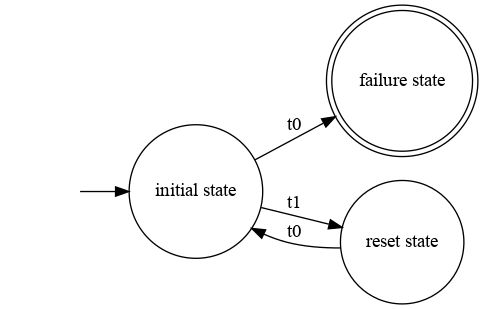
\includegraphics[scale=0.6]{graph/TimeoutCheck}
    \caption{\gls{fsm} for the timeout check}
    \label{timeoutcheck}
\end{figure}

The figure~\ref{timeoutcheck} shows how we designed this test. Transition are, of course, complex so we only show a simplified name for them. They are quite obvious given the rest of the diagram.

\subsection{Date check}

This test verify that the system uses the correct date. With an incorrect date set, the messages sent by it to the Railnova servers will be discarded resulting in a loss of communication from this device.\\

This test uses the serial connection and make uses of Unix commands directly on the system thus this is not a black-box testing processes.\\

The most complicated part here is to get the serial connection, a lot of troubles can arrise while trying to log-in the system. Once we have a valid serial connection, we can simply issue a "date" command and parse the result. The date is updated through GPS/GSM antenna communication and this proces can take up to an hour so if the date is not set rigth (if the date appears to be in 1970), we simply wait an hour and then, issue the test again.\\

1970 is the date you get when the timestamp is not set. This is because of how Unix and timestamp systems works.

TODO
\begin{figure}
    \centering
    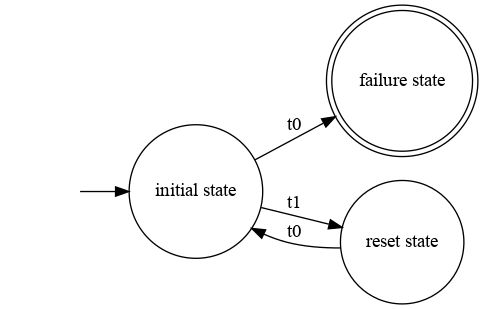
\includegraphics[scale=0.6]{graph/TimeoutCheck}
    \caption{\gls{fsm} for the date check}
    \label{datecheck}
\end{figure}

\subsection{Battery cycle}

We made some test that where not related to the \gls{rug}. One of those was able to charge a battery and then discharge it. The goal of this was measure the electrical levels all along those steps to determine wether or not the battery is working.\\

As shown in the figure~\ref{battcycle2}, we made several cycle of charge/discharge. This particular test was designed for a piece of hardware and not for a software. This is a sufficent proof to show that our system work as well for a software thant it does for hardware.

\begin{figure}
    \centering
    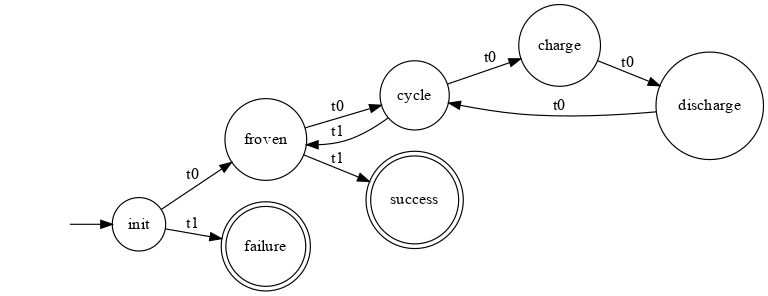
\includegraphics[scale=0.4]{graph/BatteryCycle.png}
    \caption{\gls{fsm} for the battery cycle}
    \label{battcycle2}
\end{figure}

\clearpage
\addcontentsline{toc}{section}{References}
\bibliographystyle{IEEEtran}
\bibliography{ref}{}

\clearpage
\printglossaries

\end{document}
